\documentclass{article}

\usepackage[UTF8]{ctex}
\usepackage{amsmath,amssymb}
\usepackage{geometry}
\usepackage{graphicx}
\usepackage{float}

\geometry{a4paper, margin=2.5cm}

\begin{document}

% ============================================================
\section*{深度 Q 网络（DQN）}

\subsection*{先讲一个故事}

2013 年，DeepMind 发布了一篇论文，做了一件听起来疯狂的事：用同一套代码、同一组超参数，让 AI 玩 Atari 游戏。不告诉它游戏规则，只让它看屏幕像素和分数——就像一个对说明书一无所知的小孩，坐在电视机前乱按按键。

到 2015 年，升级版打赢了 49 款游戏中的大多数，在《打砖块》《乒乓》等游戏上达到并超越人类水平。这个 AI 叫 \textbf{DQN（Deep Q-Network）}。

在 DQN 之前，深度神经网络和强化学习之间有一道公认的鸿沟：\textbf{训练不稳定}。用神经网络逼近 $Q$ 值函数，训练往往发散。DQN 用两个优雅的工程技巧彻底解决了这个问题。

\textbf{本章的核心问题}：Q-learning 已经够好了，为什么还需要 DQN？

% ============================================================
\section*{为什么 Q 表不够——维度灾难}

回顾 Q-learning 的更新规则：
\[
Q(s,a) \leftarrow Q(s,a) + \alpha\!\left[r + \gamma \max_{a'} Q(s',a') - Q(s,a)\right]
\]

这个算法需要一张 \textbf{Q 表}：对每一个状态-动作对 $(s,a)$ 存一个数值。在离散格子世界里，这没问题。但在 CartPole 里，状态是 4 个连续数字（小车位置、速度、杆角度、角速度），Q 表有无穷多行。

即使强行离散化，问题也没解决：

\[
\begin{array}{c|c}
\text{每维度格数} & \text{CartPole Q 表条目数（4维，2个动作）} \\
\hline
b = 10  & 10^4 \times 2 = 20{,}000 \\
b = 20  & 20^4 \times 2 = 320{,}000 \\
b = 100 & 100^4 \times 2 = 200{,}000{,}000 \\
\end{array}
\]

Atari 游戏的状态是 $84 \times 84 \times 4$ 的灰度图像帧，Q 表的条目数约为 $256^{84\times 84\times 4}$——连写都写不下（如图~\ref{fig:qtable}）。

\begin{figure}[H]
  \centering
  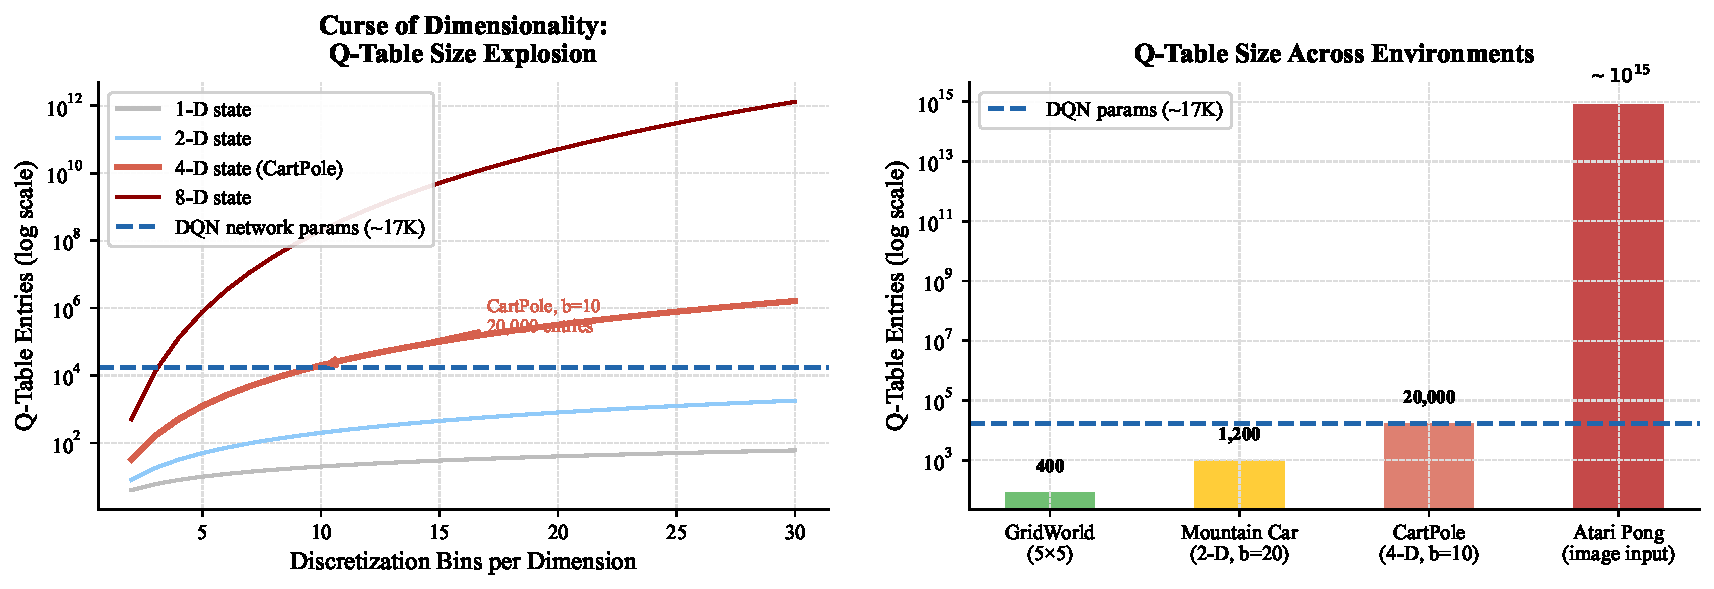
\includegraphics[width=0.95\textwidth]{fig1_qtable_motivation.pdf}
  \caption{维度灾难：Q 表大小随状态维度和离散化精度指数爆炸，远超一个小型神经网络的参数量。}
  \label{fig:qtable}
\end{figure}

\textbf{出路}：不要存一张表，改用一个\textbf{函数}来拟合 $Q(s,a)$。

% ============================================================
\section*{创新一：用神经网络逼近 $Q$ 值}

\subsection*{从 Q 表到 Q 网络}

用参数为 $\theta$ 的神经网络代替 Q 表：
\[
\boxed{Q(s, a;\, \theta) \approx Q^*(s, a)}
\]

网络的输入是状态 $s$，输出是\textbf{所有动作的 Q 值向量}——一次前向传播，同时得到所有动作的估值：
\[
a^* = \arg\max_{a}\, Q(s, a;\, \theta)
\]

\subsection*{损失函数}

训练目标是让预测值逼近 Bellman 目标，损失为均方误差：
\[
\boxed{\mathcal{L}(\theta) = \mathbb{E}_{(s,a,r,s') \sim \mathcal{D}}\!\left[\Bigl(r + \gamma \max_{a'} Q(s', a';\, \theta^-) - Q(s, a;\, \theta)\Bigr)^2\right]}
\]

其中 $\mathcal{D}$ 是经验数据集，$\theta^-$ 是目标网络参数（后面详述）。

\subsection*{直接训练的两个致命问题}

如果朴素地用每步转换 $(s, a, r, s')$ 做梯度下降，会遇到：
\begin{itemize}
  \item \textbf{问题一——时序相关性}：连续两帧的状态极度相似，梯度估计方差大，训练不稳定；
  \item \textbf{问题二——移动靶}：损失函数中的目标 $r + \gamma\max_{a'}Q(s',a';\theta)$ 本身随 $\theta$ 变化——追一个会跑的靶，Q 值容易发散。
\end{itemize}

DQN 的后两个创新分别精确地解决这两个问题。

% ============================================================
\section*{创新二：经验回放（Experience Replay）}

\subsection*{问题：时序相关}

在线 Q-learning 每走一步就立刻更新网络。相邻两步的状态高度相关（小车向右倾 $\to$ 下一帧小车还在偏右），违反了随机梯度下降对样本独立同分布（i.i.d.）的假设，导致梯度方差大、训练震荡。

\subsection*{解法：回放缓冲区}

把每步经验 $(s, a, r, s', \mathrm{done})$ 存入先进先出的\textbf{回放缓冲区} $\mathcal{D}$（容量 $N$），训练时从中\textbf{随机均匀采样}一个小批量：

\[
\boxed{\{(s_i, a_i, r_i, s_i')\}_{i=1}^{B} \;\sim\; \mathrm{Uniform}(\mathcal{D})}
\]

\subsection*{为什么有效}

\begin{itemize}
  \item \textbf{打破时序相关}：随机采样使批次内样本近似 i.i.d.，满足梯度下降假设；
  \item \textbf{提高数据利用率}：同一条经验可被反复采样，相比在线学习不浪费；
  \item \textbf{稳定梯度}：批量大小 $B$ 越大，梯度方差越小。
\end{itemize}

消融实验如图~\ref{fig:replay} 所示：去掉经验回放后，训练曲线方差显著增大，收敛更慢。

\begin{figure}[H]
  \centering
  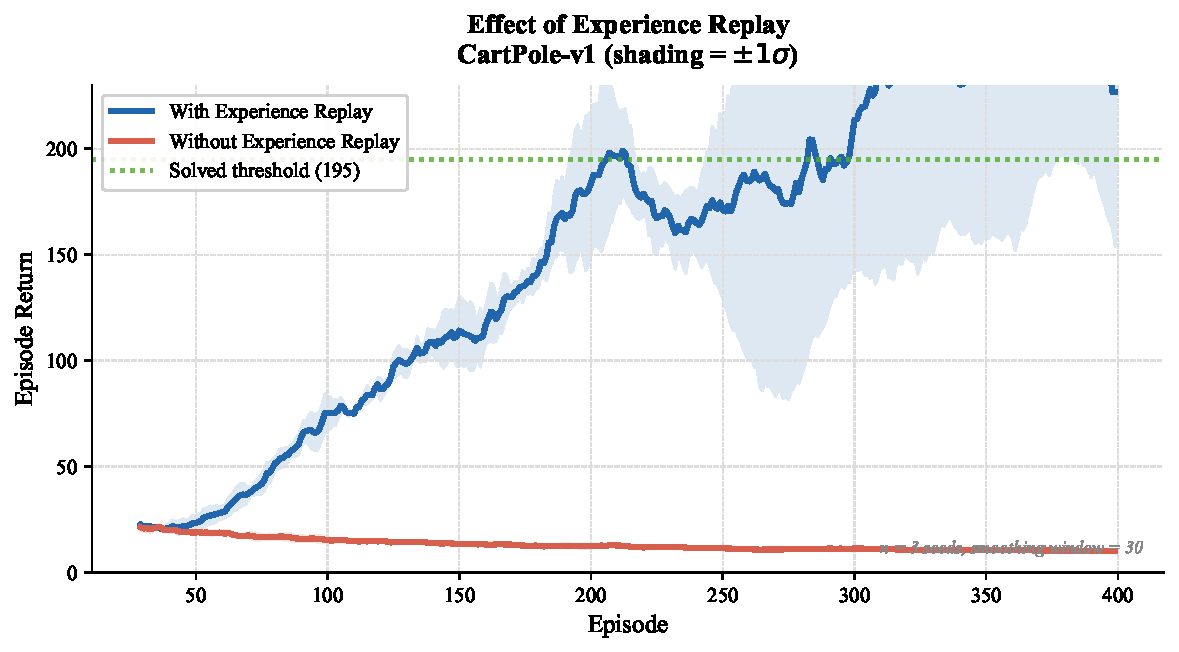
\includegraphics[width=0.88\textwidth]{fig2_replay_comparison.pdf}
  \caption{经验回放的消融实验（CartPole-v1，3 个随机种子，阴影为 $\pm 1\sigma$）。有经验回放的版本收敛更快、方差更小。}
  \label{fig:replay}
\end{figure}

% ============================================================
\section*{创新三：目标网络（Target Network）}

\subsection*{问题：移动靶}

朴素 DQN 的损失两边都含 $\theta$：
\[
\mathcal{L}(\theta) = \mathbb{E}\!\left[\Bigl(\underbrace{r + \gamma \max_{a'} Q(s', a';\, \theta)}_{\text{目标}} - \underbrace{Q(s, a;\, \theta)}_{\text{预测}}\Bigr)^2\right]
\]

每次梯度更新让预测值向目标靠近，但目标本身也随 $\theta$ 同步改变。这是\textbf{追移动靶}——更新一个 Q 值会间接拉动其他 Q 值，引发连锁不稳定，最终 Q 值发散。

\subsection*{解法：冻结目标网络}

维护两个网络：
\begin{itemize}
  \item \textbf{在线网络} $Q(s,a;\theta)$：每步梯度更新，用于选择动作；
  \item \textbf{目标网络} $Q(s,a;\theta^-)$：参数\textbf{冻结}，只参与 Bellman 目标的计算，每隔 $C$ 步从在线网络硬同步一次：
\end{itemize}
\[
\boxed{\theta^- \;\leftarrow\; \theta \quad \text{（每隔 } C \text{ 步同步，其余时刻冻结）}}
\]

损失函数变为：
\[
\mathcal{L}(\theta) = \mathbb{E}\!\left[\Bigl(\underbrace{r + \gamma \max_{a'} Q(s', a';\, \theta^-)}_{\text{固定目标（短期内不动）}} - Q(s, a;\, \theta)\Bigr)^2\right]
\]

\textbf{直觉}：把「每步都在移动的靶」换成了「每 $C$ 步挪一次的靶」——短期内靶静止，训练稳定得多。$C$ 越大靶越稳，但 $\theta^-$ 也越滞后，通常取 $C \in [10, 1000]$。

消融实验如图~\ref{fig:target} 所示。

\begin{figure}[H]
  \centering
  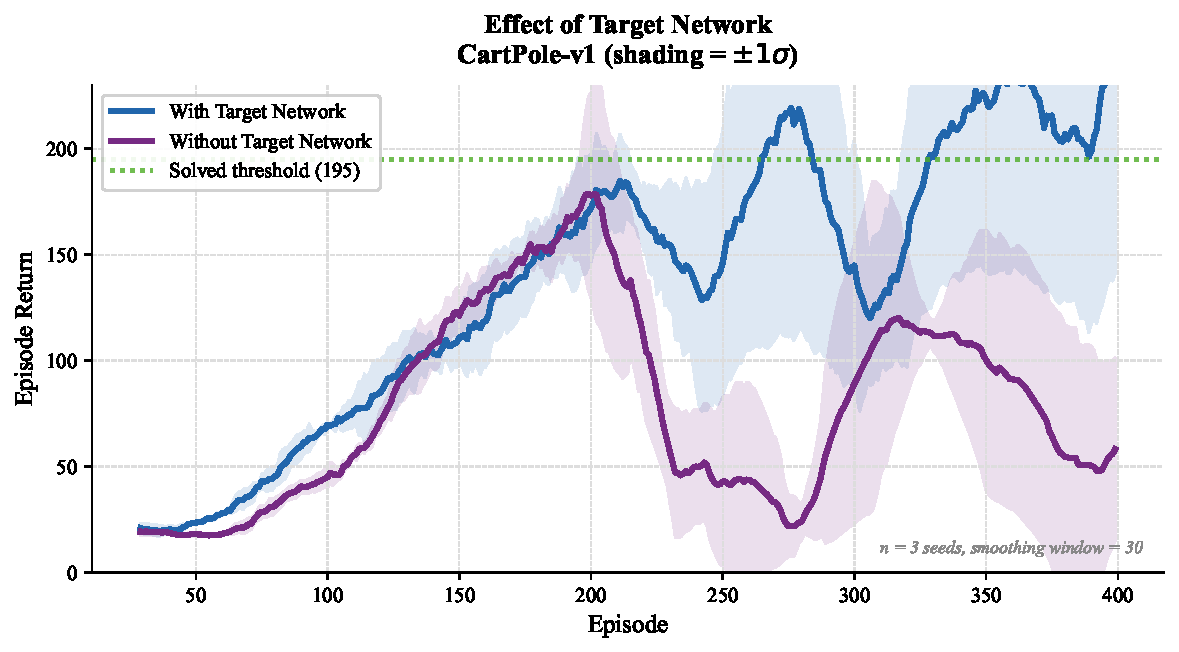
\includegraphics[width=0.88\textwidth]{fig3_target_comparison.pdf}
  \caption{目标网络的消融实验（CartPole-v1，3 个随机种子，阴影为 $\pm 1\sigma$）。无目标网络时，训练曲线更不稳定，种子间方差更高。}
  \label{fig:target}
\end{figure}

% ============================================================
\section*{完整 DQN 算法}

综合三个创新：

\begin{enumerate}
  \item \textbf{初始化}：回放缓冲区 $\mathcal{D}$（容量 $N$），在线网络参数 $\theta$，目标网络 $\theta^- \leftarrow \theta$，探索率 $\varepsilon$；
  \item \textbf{每个 episode}，对每步 $t$：
  \begin{enumerate}
    \item 以 $\varepsilon$-贪心选动作：
          \[a_t = \begin{cases} \text{随机} & \text{以概率 } \varepsilon \\ \arg\max_{a} Q(s_t, a;\theta) & \text{以概率 } 1-\varepsilon \end{cases}\]
    \item 执行 $a_t$，观测 $r_t$、$s_{t+1}$；将 $(s_t, a_t, r_t, s_{t+1}, \mathrm{done})$ 存入 $\mathcal{D}$；
    \item 从 $\mathcal{D}$ 随机采 $B$ 条，计算 Bellman 目标：
          \[y_i = \begin{cases} r_i & \text{若终止} \\ r_i + \gamma \max_{a'} Q(s_i', a';\theta^-) & \text{否则} \end{cases}\]
    \item 梯度更新：$\displaystyle\theta \leftarrow \theta - \alpha \nabla_\theta \frac{1}{B}\sum_{i=1}^B \bigl(y_i - Q(s_i, a_i;\theta)\bigr)^2$；
    \item 每 $C$ 步执行：$\theta^- \leftarrow \theta$。
  \end{enumerate}
\end{enumerate}

\textbf{三个创新一句话总结}：

\[
\begin{array}{l|l|l}
\textbf{问题} & \textbf{创新} & \textbf{核心操作} \\
\hline
\text{状态空间无限大} & \text{神经网络逼近} & Q(s,a;\theta) \approx Q^*(s,a) \\[4pt]
\text{样本时序相关} & \text{经验回放} & (s,a,r,s') \sim \mathrm{Uniform}(\mathcal{D}) \\[4pt]
\text{目标不稳定} & \text{目标网络} & \theta^- \leftarrow \theta \;\text{每 } C \text{ 步}\\
\end{array}
\]

% ============================================================
\section*{DQN 在 RL 体系中的位置}

DQN 是深度强化学习的起点，往前承接经典 RL，往后开启整条深度 RL 主线：

\begin{enumerate}
  \item \textbf{从表格到网络}：Q-learning（表格，离散小状态）$\to$ DQN（神经网络，连续高维状态），更新规则完全相同，只换了函数近似器；
  \item \textbf{经验回放的深远影响}：固定数据集 + 离线学习，就是\textbf{离线强化学习（Offline RL）}的核心范式——后续 CQL、IQL 等算法的数据均来自某种形式的回放缓冲区；
  \item \textbf{目标网络的演化}：Hard update $\theta^- \leftarrow \theta$ $\to$ Soft（Polyak）update $\theta^- \leftarrow (1-\tau)\theta^- + \tau\theta$，后者被 DDPG、TD3、SAC 广泛沿用；
  \item \textbf{下一步}：Double DQN（解耦动作选择与评估，缓解 Q 值高估）、Dueling DQN（将 Q 分解为状态价值 $V$ 与优势函数 $A$）——都是在 DQN 框架上的精准改进。
\end{enumerate}

\subsection*{参考资料}

\begin{enumerate}
  \item Mnih, V., et al.\ (2013). Playing Atari with Deep Reinforcement Learning. \textit{NeurIPS Deep Learning Workshop}.
  \item Mnih, V., et al.\ (2015). Human-level control through deep reinforcement learning. \textit{Nature}, 518, 529--533.
  \item Sutton, R.\,S.\ \& Barto, A.\,G.\ (2018). \textit{Reinforcement Learning: An Introduction} (2nd ed.). Chapters 9--10.
  \item 动手学强化学习（Hands-on-RL）. 第 7 章：DQN 算法.
\end{enumerate}

\end{document}
